\documentclass[a4paper,12pt]{article}

\usepackage{cmap}                   % правильный PDF (на первом месте)
\usepackage{ucs}                    % unicode
\usepackage[utf8x]{inputenc}
\usepackage[english,russian]{babel}
\usepackage[pdftex]{graphicx}
\usepackage[force]{feynmp-auto}

\unitlength=1mm
\graphicspath{{figures/}}
\PrerenderUnicode{ая}

\begin{document}

\begin{center}
  \Large\bf {Реакция перезарядки $dp \to (pp)n$}
\end{center}

\begin{center}
  \noindent \large\textrm {В.~В.~Глаголев$^{1}$, Г.~Мартинска$^{2}$,
    Я.~Мушински$^{1, 2}$, Н~.М.~Пискунов$^{1}$, Й.~Урбан$^{2}$}
\end{center}
\vspace {0.5cm}
\small {$^{1}$ Объединенный Институт Ядерных Исследований, Дубна \\
  $^{2}$ Университет П.~Й.~Шафарика, Кошице, Словакия \\}

\begin{center} {\bf Аннотация}
\end{center}
\vspace{0.5cm} Обсуждается отношение дифференциальных поперечных
сечений перезарядки на дейтроне и нуклоне в области малых переданных
импульсов с целью оценки спинзависящей части амплитуды $np\to pn$
перезарядки.

\section{Введение}
В последнее время прошли дискуссии на семинарах, посвященных вопросам
извлечения информации о cечениях спинзависящей части $np$ - рассеяния
из реакций перезарядки на дейтроне. Возобновился интерес к подобным
исследованиям, особенно в связи с возможностями ускорения дейтронов с
энергией выше 1~ГэВ на нуклон на Нуклотроне ЛВЭ ОИЯИ.  Продолжают
обсуждаться старые идеи Померанчука и Чу ~\cite{a1} , формализованные
в работах Дина и др. Эти формулы выведены в определенных
предположениях, а именно, при справедливости импульсного приближения и
условия полноты.  В работе Ледницкого и др.~\cite{a2} показано, что
при релятивистских энергиях эти предположения оправданы .  Кроме того,
при экспериментальном исследовании взаимодействия в конечном состоянии
(ВКС)оказалось, что к эффекту ВКС очень чувствительны асимметрии
распределений по углу $\alpha=(\vec{p_s}\vec{q})$ , где $\vec{p_s}$ -
импульс спектатора в системе покоя дейтрона, а $\vec{q}$ - трехмерная
передача от падающего нуклона к рассеянному. В работах ~\cite{a3,a4}
было показано, что в области |t|<0.1~(ГэВ/c)$^{2}$ и импульсов
спектаторов меньших 0.1~ГэВ/с асимметрии, вызванные ВКС, практически
отсутствуют, что хорошо видно как для прямого развала, так и для
развала дейтрона с перезарядкой на рис.~\ref{f_asym}.

\begin{figure}[!h]
  \centering
  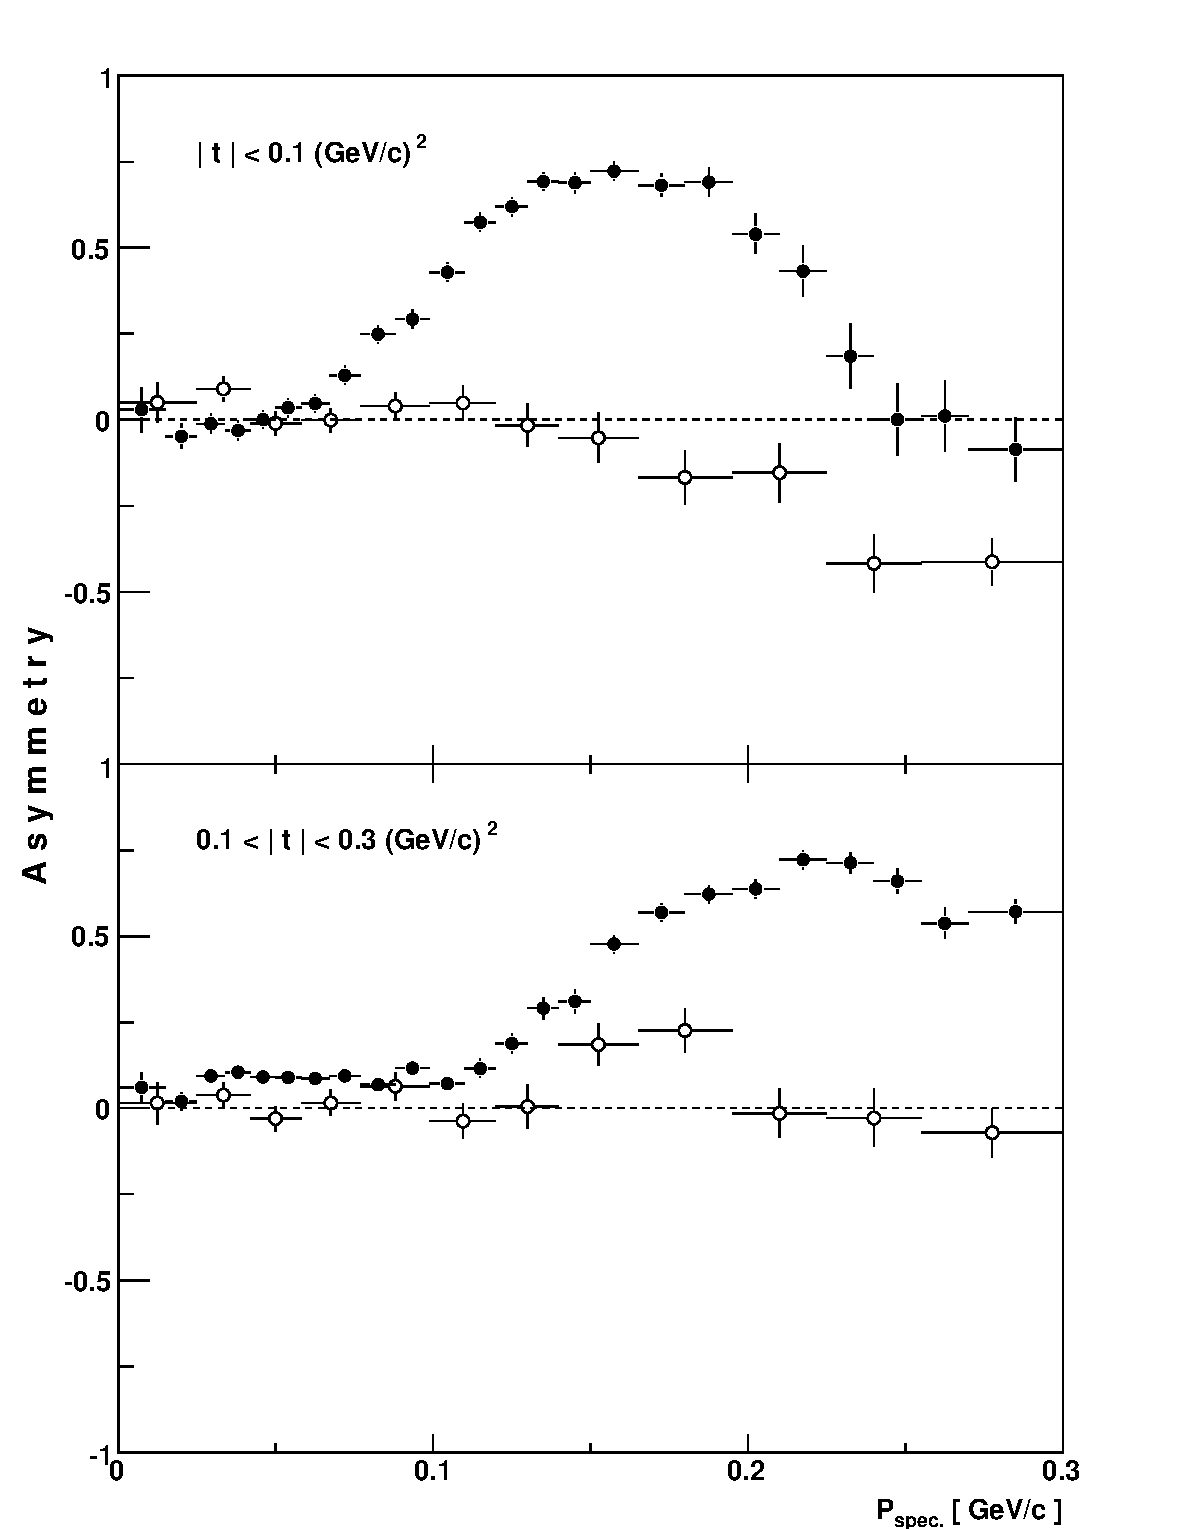
\includegraphics[width=0.88\textwidth]{fig_asym.pdf}
  \caption {Асимметрия по углу $\alpha=(\vec{p_s}\vec{q})$ , где
    $\vec{p_s}$ - импульс спектатора в системе покоя дейтрона, а
    $\vec{q}$ - трехмерная передача от падающего нуклона к
    рассеянному. Пустые кружки - реакция перезарядки, сплошными
    кружками обозначены данные для прямого развала.}
  \label{f_asym}
\end{figure}

Это важно учитывать при продвижении в область более высоких энергий, в
которой отсутствуют экспериментальные данные по $np$ - рассеянию.
Выше 1~ГэВ имеются лишь предварительные результаты группы Дельта-сигма
~\cite{a5}. Кроме того, в связи с развитием поляризационных методов
исследований в Дубне (Нуклотрон) и Юлихе (COSY), существенно
расширяются возможности восстановления амплитуд и фаз
нуклон-нуклонного рассеяния в области энергий до и выше 1 ГэВ'а. В
связи со сказанным, мы критически переосмысливаем представление
экспериментальных данных по изучению реакции перезарядки на дейтроне
$dp\to(pp)n$ , полученных на водородной пузырьковой камере ~\cite{a6}.

\section{Эксперимент}
Экспериментальный материал был получен с помощью 100-см водородной
пузырьковой камеры на синхрофазотроне ЛВЭ ОИЯИ.  Камера была облучена
выведенным из ускорителя пучком дейтронов импульса 3.35 ГэВ/с. После
стандартной процедуры просмотра, измерений и идентификации была
получена в условиях $4\pi$-геометрии информация о~17~реакциях,
представленных в таблице~\ref{t_channels}.

\begin{table}[!hbp]
  \begin{center}
    \begin{tabular}{|r|l|r|} \hline &реакция&число событий \\ \hline
      1.&$ppn$&102778\\ \hline 2.&$ppn\pi^{0}$&31295 \\ \hline
      3.&$p\pi^{+}nn$&65284 \\ \hline 4.&$dp$&16184\\ \hline
      5.&$dp\pi^{0}$&3950\\ \hline 6.&$dp\pi^{0}\pi^{0}$&1839\\ \hline
      7.&$d\pi^{+}n$&4963\\ \hline 8.&$d\pi^{+}n\pi^{0}$&1843\\ \hline
      9.&$\pi^{+}\pi^{+}nn$&315\\ \hline 10.&$ppp\pi^{-}$&5487\\
      \hline 11.&$ppp\pi{-}\pi^{0}$&167\\ \hline
      12.&$ppp\pi^{-}\pi^{0}\pi^{0}$&67\\ \hline
      13.&$pp\pi^{+}\pi^{-}n$&1163\\ \hline
      14.&$pp\pi^{+}\pi^{-}n\pi^{0}$&49\\ \hline
      15.&$dp\pi^{+}\pi^{-}$&576\\ \hline
      16.&$dp\pi^{+}\pi^{-}\pi^{0}$&39\\ \hline
      17.&$dp\pi^{+}\pi^{-}\pi^{0}\pi^{0}$&1414\\ \hline
    \end{tabular}
    \caption{Перечень наблюдаемых реакций} \label{t_channels}
  \end{center}
\end{table}

Видно, что около половины всех событий составляла реакция безмезонного
развала дейтрона $dp\to ppn$.  Эту реакцию можно разделить на два
класса - прямой развал $dp\to (pn)p$ и перезарядку $dp\to (pp)n$.  К
перезарядке отнесены события, в которых самым быстрым из вторичных
нуклонов в системе покоя дейтрона являлся нейтрон. Таких событий было
$17512$, что соответствовало поперечному сечению $( 5.85 \pm 0.05 )$
мбн. При этом миллибарн-эквивалент события определялся исходя из
полного сечения $dp$ - заимодействий ~\cite{a7} с учетом потерь
событий упругого $dp$ - рассеяния.  Систематическая ошибка, связанная
с оценкой потерь в упругом $dp$ - рассеянии составляла около $4 \%$.

Заметим, что это сечение включает в себя часть событий квази $pp$ -
рассеяния с образованием промежуточной $\Delta$-изобары. Ниже мы
обсудим соответствующую поправку. Инвариантную величину t
экспериментально определяем как переданный $4$-импульс от протона
мишени к нейтрону в лабораторной системе координат.

Напомним некоторые из теоретических формул
~\cite{a8,a9}. Дифференциальное поперечное сечение $np\to pn$
рассеяния может быть представлено в виде суммы спин-независящей
(индекс SI) и спин-зависящей (индекс SD) частей:
\begin{displaymath}
  (d\sigma/dt)_{np\rightarrow pn}=(d \sigma /dt)^{SI}_{np\rightarrow
    pn} + (d \sigma /dt)^{SD}_{np\rightarrow pn}
\end{displaymath}
Амплитуда элементарной реакции перезарядки $pn \to np$ может быть
записана как:
\begin{displaymath}
  f_{ce}=a_{ce}+b_{ce} (\sigma \vec{n})( \sigma _{i}\vec{n})
  +c_{ce}[(\sigma \vec{n})+( \sigma _{i} \vec{n})]+d_{ce} [(\sigma
    \vec{m})( \sigma _{i}\vec{m})]+e_{ce} [(\sigma \vec{l})( \sigma
    _{i}\vec{l})],
\end{displaymath}
где операторы $\sigma $ и $\sigma _i$ являются матрицами Паули
падающей частицы (нейтрон) и i-того нуклона (протон), коэффициенты
$a_{ce}$, $b_{ce}$, $c_{ce}$, $d_{ce}$, $e_{ce}$ являются комплексными
функциями энергии и угла рассеяния взаимодействующих частиц.
\begin{displaymath}
  \vec{n}=\frac{\vec{k}\times\vec{k'}}{|\vec{k}\times\vec{k'}|},~~
  \vec {m}=\frac{\vec{k'}-\vec{k}}{|\vec{k'}-\vec{k}|},~~
  \vec{l}=\frac{\vec{k'}+\vec{k}}{|\vec{k'}+\vec{k}|}\,
\end{displaymath}
$ \vec{k}$ и $\vec{k'}$ - импульсы падающего и рассеянного нуклонов в
CMS.

Заметим, что имеются по крайней мере два инвариантных относительно
обращения времени и пространства типа представления матрицы рассеяния
- это представление Гольдбергера ~\cite{a10} и представление
Быстрицкого, Легара, Винтерница ~\cite{a11}, которые равнозначны.

Для спин-независящей и спин-зависящей частей дифференциального
поперечного сечения получаем:
\begin{displaymath}
  (d \sigma /dt)^{SI}_{np\rightarrow pn} = (\pi /p^{2}){\vert
  }a_{ce}{\vert }^{2}
\end{displaymath}
\begin{displaymath}
  (d \sigma /dt)^{SD}_{np\rightarrow pn} =(\pi/p^{2})[ \vert b_{ce}
    \vert ^{2}+ \vert c_{ce} \vert ^{2}+ \vert d_{ce} \vert ^{2}+ \vert
    e_{ce} \vert ^{2}],
\end{displaymath}
где p - импульс в системе центра масс NN-системы.

Соотношение между поперечным сечением периферической перезарядки на
дейтроне $dp \to (pp)n$ и процессом элементарной перезарядки $pn \to np$
обсуждалось во многих работах. Математический формализм, развитый
в ~\cite{a8, a9} позволяет в рамках импульсного приближения записать
дифференциальное поперечное сечение перезарядки на дейтроне в виде:
\begin{displaymath}
  (d \sigma /dt)_{dp\rightarrow(pp)n} = [1-S(t)] (d \sigma
  /dt)^{SI}_{np\rightarrow pn} + [1-1/3S(t)] (d \sigma
  /dt)^{SD}_{np\rightarrow pn}
\end{displaymath}
Здесь $S(t)= \int [\Psi(r)]^{2}e^{-iqr}d^{3}r$ обозначает форм-фактор
дейтрона и $q^2 = t$~квадрат четырехмерного переданного импульса. Из
этой формулы следует, что при нулевом переданном импульсе от
протона-мишени к нейтрону, т.е. при угле рассеяния $180^{\circ}$ в
ситеме центра масс из за того, что S(0)=1, дифференциальное поперечное
сечение равно:
\begin{displaymath}
  (d \sigma /dt)_{dp\rightarrow(pp)n} = 2/3 (d \sigma
  /dt)^{SD}_{np\rightarrow pn}
\end{displaymath}

Таким образом, реакция перезарядки неполяризованного дейтрона на
неполяризованном протоне-мишени при нулевой передаче (t=0) полностью
определяется спин-зависящей частью элементарного $np \to pn$ рассеяния
назад в~сци~($180^{\circ}$). То есть, дейтрон выступает как спиновый
фильтр. Следует заметить, что этот результат остается справедливым и
при учете D-состояния дейтрона ~\cite{a2}.

В условиях коллинеарной кинематики $\vert c_{ce}\vert ^2 = sin^2
\theta =0$ и $\vert b_{ce}-e_{ce}\vert ^2 = sin^2 \theta = 0$, т.е.
для рассеяния назад (перезарядки) получим:
\begin{displaymath}
  (d \sigma /dt)_{dp\rightarrow(pp)n} = 2/3 (\pi/p^{2})[ 2\vert b_{ce}%
    \vert ^{2}+ \vert d_{ce} \vert ^{2}].
\end{displaymath}

Таким образом, изучение процесса $dp\to (pp)n$ при малых переданных
импульсах позволяет оценить спин-зависящую часть элементарной $np\to pn$
реакции, то есть сумму амплитуд $2\vert b_{ce}\vert ^2+\vert d_{ce}\vert ^2$.

Из наших экспериментальных данных мы оцениваем величину
дифференциального поперечного сечения для перезарядки на дейтроне при
$t = 0$ и сравниваем ее с имеющимися в литературе данными по этой
величине для $np\to pn$ рассеяния при той же энергии. Самыми близкими
по энергии данными являются измерения на ускорителе Сатурн, сделанные
Бизардом и др.~\cite{a12,a13}.

\begin{figure}[hp]
  \centering
  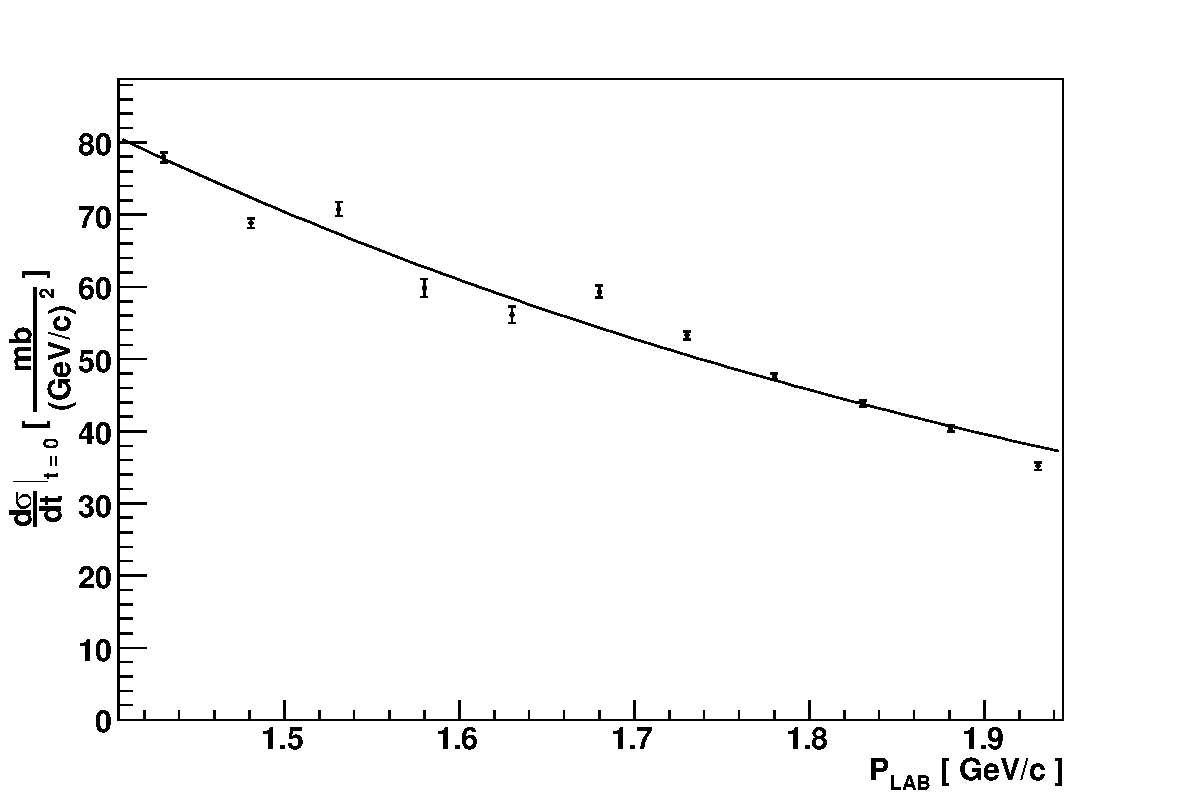
\includegraphics[width=0.75\textwidth]{fig_bizard.pdf}
  \caption {Экстраполяция данных Сакле к $t = 0$.}
  \label{f_biz}
\end{figure}

На рис.~\ref{f_biz} мы приводим дифференциальные поперечные сечения из
этой работы в области импульсов $(1.4 - 1.95)$ ГэВ/с
экстраполированные к $t = 0$ выражением
\begin{displaymath}
  d\sigma/dt = a \exp(bt+ct^2).
\end{displaymath}
Экспоненциальный фит этих значений дал для нашей энергии 1.675 ГэВ/с
на нуклон величину $d\sigma/dt|_{t=0} = 54.7 \pm
0.2$мбн/(ГэВ/с)$^{2}$. К полученному значению мы и будем в дальнейшем
относить нашу оценку дифференциального поперечного сечения для
квазиупругой $dp\to(pp)n$ перезарядки при $t = 0$.  Заметим, что
систематическая ошибка в данных Бизарда и др.  составляла $5\%$.

\begin{figure}[!h]
  \centering
  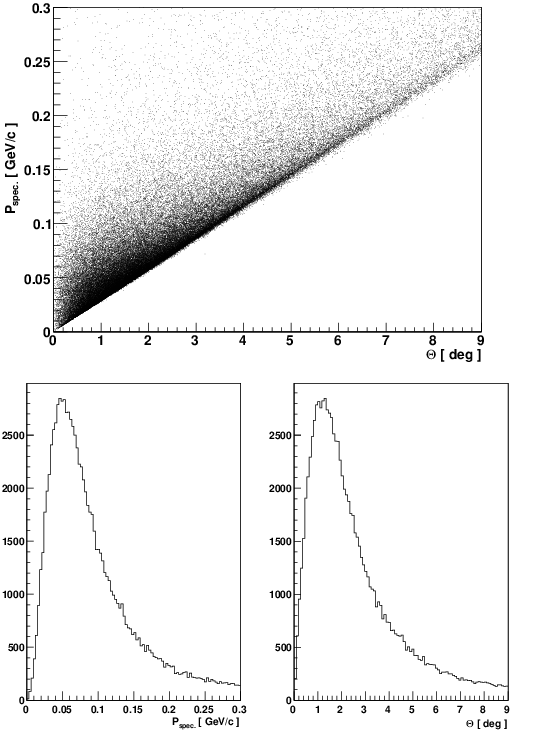
\includegraphics[width=0.78\textwidth]{fig_theta_p.png}
  \caption {Диаграмма: импульс нуклона-спектатора в системе покоя
    дейтрона в зависимости от угла его вылета в лабораторной системе
    координат.  Под диаграммой показаны ее проекции. Масштаб
    распределений выбран таким, чтобы показать их подобие.}
  \label{f_tp}
\end{figure}

Воспользуемся кинематической корреляцией между полярным углом вылета
нуклона-спектатора в лабораторной системе координат и его импульсом в
системе покоя дейтрона, рис.~\ref{f_tp}

Видно, что при углах меньших ~5 градусов лежит основная часть событий,
соответствующих квазинуклонному рассеянию. В случае $t = 0$ два
протона в лабораторной системе координат имеют практически одинаковые
импульсы $\vec{p}_1 = \vec{p}_2 = (1/2)\vec{p}_d$. Для набора пар
протонов, попадающих в конус с раствором~$5^{\circ}$, строится
распределение $d\sigma/dt$ с учетом миллибарн-эквивалента и поправки
на поток, равной отношению полного числа спектаторных нуклонов к числу
спектаторов в конусе.

В связи с заметным вкладом событий с промежуточной $\Delta$-изобарой
~\cite{a14,a4}, основная часть которых является следствием квази-рр
столкновений, идущих через $\Delta^{++}$ и $\Delta^{+}$- изобары
(см. диаграммы a) и b) на рис.~\ref{f_feynman}), необходимо было бы
ввести поправку на квази-протонные столкновения. \\ \\

\begin{figure}[!h]
  \begin{center}

    \begin{fmffile}{ppn_fmf}
      % pp1
      \parbox{56mm} {
        \begin{fmfgraph*}(54,27)
          \fmfset{arrow_len}{4mm}\fmfset{arrow_ang}{8}

          \fmfleft{iA,iB}
          \fmfright{o1,o2,o3}
          \fmflabel{$d$}{iA}
          \fmflabel{$p$}{iB}
          \fmflabel{$p$}{o3}
          \fmflabel{$n$}{o2}
          \fmflabel{$p$}{o1}

          \fmf{fermion,tension=1.0}{iA,v1} % default tension=1.0
          \fmf{fermion,tension=1.0}{v2,o1}
          \fmf{fermion,tension=1.0}{v2,o2}
          \fmf{fermion,tension=1.0}{iB,v3,o3}

          \fmf{fermion,tension=1.5,label=$n$}{v1,v2}
          \fmf{fermion,tension=0.2,lab.side=left,label=$p$}{v1,v3}
          \fmf{fermion,tension=0.1,lab.side=left,label=$\Delta^{+}$}{v3,v2}

          \fmfblob{0.06w}{v1}
          \fmfdot{v2,v3}
          \fmf{dbl_plain_arrow}{iA,v1}
          \fmffreeze
          \fmf{dbl_plain_arrow}{v3,v2}
        \end{fmfgraph*}
      }
      % pp2
      \quad
      \parbox{56mm} {
        \begin{fmfgraph*}(54,27)
          \fmfset{arrow_len}{4mm}\fmfset{arrow_ang}{8}

          \fmfleft{iA,iB}
          \fmfright{o1,o2,o3}
          \fmflabel{$d$}{iA}
          \fmflabel{$p$}{iB}
          \fmflabel{$n$}{o3}
          \fmflabel{$p$}{o2}
          \fmflabel{$p$}{o1}

          \fmf{fermion,tension=1.0}{iA,v1} % default tension=1.0
          \fmf{fermion,tension=1.0}{v2,o1}
          \fmf{fermion,tension=1.0}{v2,o2}
          \fmf{fermion,tension=1.0}{iB,v3,o3}

          \fmf{fermion,tension=1.5,label=$n$}{v1,v2}
          \fmf{fermion,tension=0.2,lab.side=left,label=$p$}{v1,v3}
          \fmf{fermion,tension=0.1,lab.side=left,label=$\Delta^{++}$}{v3,v2}

          \fmfblob{0.06w}{v1}
          \fmfdot{v2,v3}
          \fmf{dbl_plain_arrow}{iA,v1}
          \fmffreeze
          \fmf{dbl_plain_arrow}{v3,v2}
        \end{fmfgraph*}
      }
      \begin{center}
        % \vspace{5mm}
        \texttt{a)} \hspace{56mm} \texttt{b)}
      \end{center}
      % np1
      \vspace{10mm}
      \parbox{56mm} {
        \begin{fmfgraph*}(54,27)
          \fmfset{arrow_len}{4mm}\fmfset{arrow_ang}{8}

          \fmfleft{iA,iB}
          \fmfright{o1,o2,o3}
          \fmflabel{$d$}{iA}
          \fmflabel{$p$}{iB}
          \fmflabel{$n$}{o3}
          \fmflabel{$p$}{o2}
          \fmflabel{$p$}{o1}

          \fmf{fermion,tension=1.0}{iA,v1} % default tension=1.0
          \fmf{fermion,tension=1.0}{v2,o1}
          \fmf{fermion,tension=1.0}{v2,o2}
          \fmf{fermion,tension=1.0}{iB,v3,o3}

          \fmf{fermion,tension=1.5,label=$p$}{v1,v2}
          \fmf{fermion,tension=0.2,lab.side=left,label=$n$}{v1,v3}
          \fmf{fermion,tension=0.1,lab.side=left,label=$\Delta^{+}$}{v3,v2}

          \fmfblob{0.06w}{v1}
          \fmfdot{v2,v3}
          \fmf{dbl_plain_arrow}{iA,v1}
          \fmffreeze
          \fmf{dbl_plain_arrow}{v3,v2}
        \end{fmfgraph*}
      }
      % pp2
      \quad
      \parbox{56mm} {
        \begin{fmfgraph*}(54,27)
          \fmfset{arrow_len}{4mm}\fmfset{arrow_ang}{8}

          \fmfleft{iA,iB}
          \fmfright{o1,o2,o3}
          \fmflabel{$d$}{iA}
          \fmflabel{$p$}{iB}          \fmflabel{$p$}{o3}
          \fmflabel{$n$}{o2}
          \fmflabel{$p$}{o1}

          \fmf{fermion,tension=1.0}{iA,v1} % default tension=1.0
          \fmf{fermion,tension=1.0}{v2,o1}
          \fmf{fermion,tension=1.0}{v2,o2}
          \fmf{fermion,tension=1.0}{iB,v3,o3}

          \fmf{fermion,tension=1.5,label=$p$}{v1,v2}
          \fmf{fermion,tension=0.2,lab.side=left,label=$n$}{v1,v3}
          \fmf{fermion,tension=0.1,lab.side=left,label=$\Delta^{\circ}$}{v3,v2}

          \fmfblob{0.06w}{v1}
          \fmfdot{v2,v3}
          \fmf{dbl_plain_arrow}{iA,v1}
          \fmffreeze
          \fmf{dbl_plain_arrow}{v3,v2}
        \end{fmfgraph*}
      }
      \begin{center}
        % \vspace{5mm}
        \texttt{c)} \hspace{56mm} \texttt{d)}
      \end{center}
    \end{fmffile}

    \caption{Диаграммы Фейнмана для реакции $dp\rightarrow ppn$ с
      участием промежуточной $\Delta$-изобары}
    \label{f_feynman}
  \end{center}
\end{figure}

На рис.~\ref{f_res} приведено сравнение распределений по
импульсам спектаторов из прямого развала и перезарядки. Виден
относительный избыток в спектре протонов-спектаторов из перезарядки,
связанный с вкладом промежуточных изобарных состояний. Из
сопоставления рисунков~\ref{f_tp} и~\ref{f_res} видно, что этот
избыток находится в области импульсов больших 0.2 ГэВ/с, т.е. вне
конуса с углом раствора до 5 градусов и не влияет на дифференциальное
сечение при $t = 0$.

Дифференциальное сечение фитированное тем же способом, как данные $np
\to pn$, приводится на рис.~\ref{f_2p}.  Экстраполяция к $t = 0$ дала
значение $d\sigma/dt|_{t=0} = 30.2 \pm 4.1$ мбн/(ГэВ/с)$^{2}$.
% Отношение этой величины к показанному выше значению из данных
% Сакле(Сатурн) $R(0)=0.55 \pm 0.08$.

\begin{figure}[hp]
  \centering
  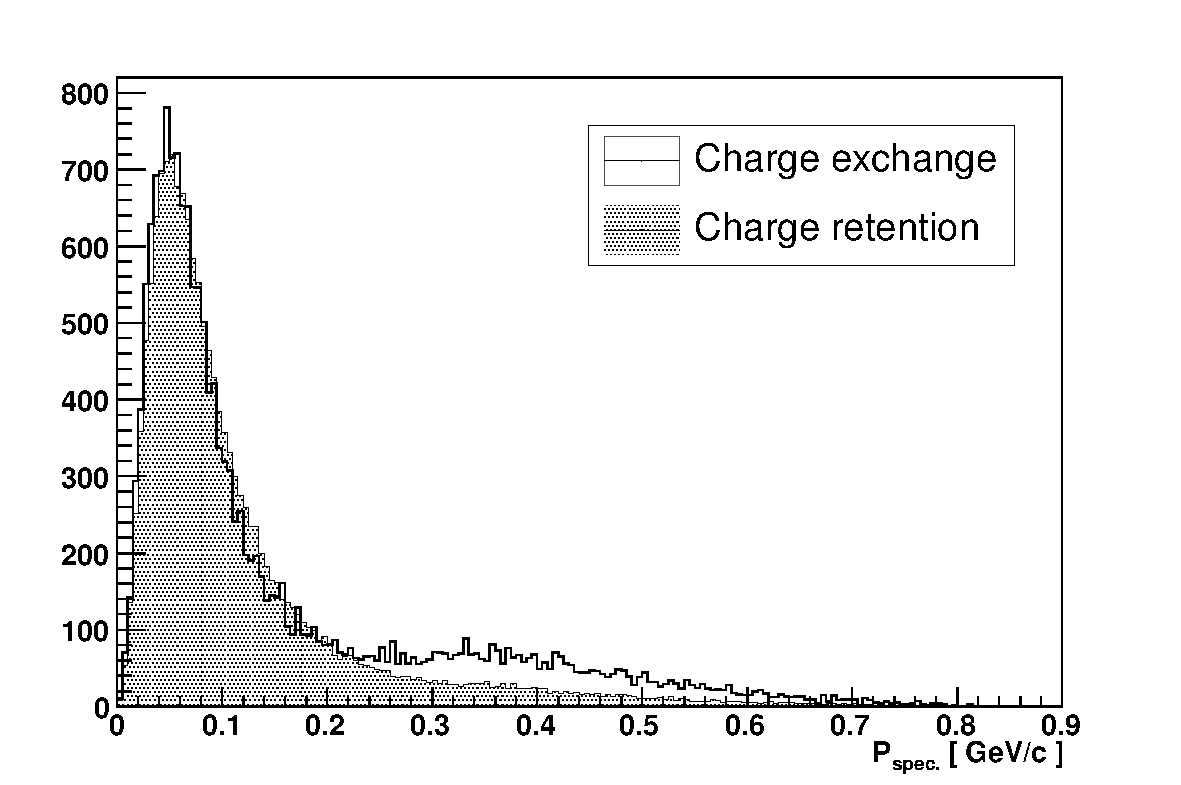
\includegraphics[width=0.90\textwidth]{fig_res.pdf}
  \caption {Импульсные распределения спектаторов из прямого канала и
    перезарядки нормированные на максимум.}
  \label{f_res}
\end{figure}

Введем отношение дифференциальных сечений для рассеяния вперед
(перезарядка) на дейтроне и протоне
$R = \frac{(d\sigma/dt)_{dp}}{(d\sigma/dt)_{np}} = 0.55\pm 0.08$.
В высказанных выше предположениях оно может быть приравнено к
$\frac{2}{3} \times \frac{(d\sigma/dt)_{np}^{SD}}{(d\sigma/dt)_{np}}$
и, соответственно, доля спиннезависящей части сечения упругой
$np\to pn$ перезарядки
$R^{ID}_{np} = \frac{(d\sigma/dt)_{np}^{SI}}{{(d\sigma/dt)_{np}^{SD}}} =
\frac{2}{3\times R} - 1 = 0.21 \pm 0.17$.

\begin{figure}[h]
  \centering
  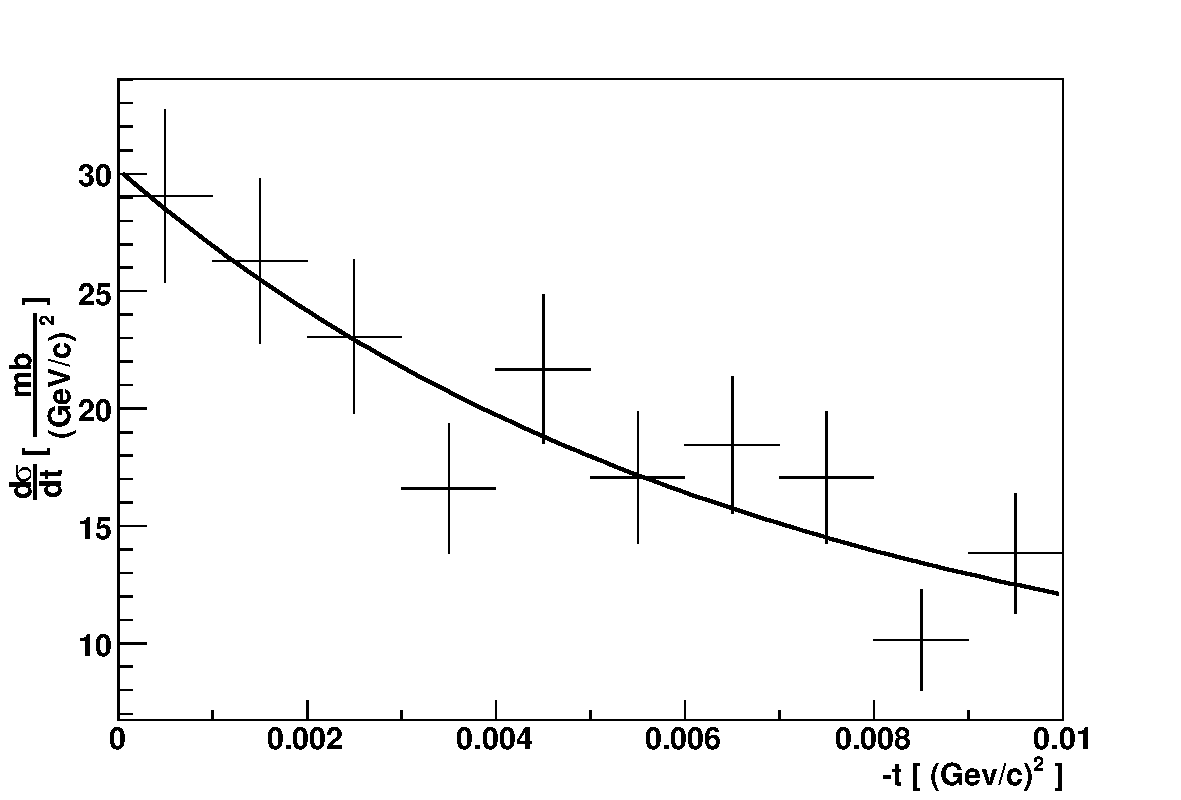
\includegraphics[width=1.00\textwidth]{fig_2p.pdf}
  \caption {Экстраполяция дифференциального сечения к $t = 0$.}
  \label{f_2p}
\end{figure}

\section {Заключение}
\begin {enumerate}
\item Критически переработано представление экспериментальных данных
  по реакции $dp\to(pp)n$, полученных на водородной пузырьковой
  камере.
\item Получено отношение дифференциальных сечений перезарядки под
  нулем градусов в реакции $dp\to(pp)n$ и $np\to pn$: $R = 0.55 \pm
  0.08$, что свидетельствует о преобладающем вкладе спин-зависящей
  части сечения $np\to pn$ рассеяния.
\item Важным является продолжение исследований в области более высоких
  энергий на установке Стрела.
\end {enumerate}

Авторы благодарят за полезные обсуждения Н.~Б.~Ладыгину, Ф.~Легара и
В.~Л.~Любошица.

Данная работа выполнена при поддержке Slovak grant agency 1/1020/04.

\begin {thebibliography} {99}
\bibitem{a1}I. Pomeranchuk, Sov. JETF 21 (1951) 1113;
  G.F.Chew,Phys.Rev. 84 (1951)710
\bibitem{a2}R.Lednicky,V.L.Lyuboshitz, V.V.Lyuboshitz, ISHEPP...2004
\bibitem{a3}B.S.Aladashvili et al, J.Phys.G: Nucl.Phys.,Vol.3,
  (1977)pp.7-20
\bibitem{a4}B.S.Aladashvili et al, J.Phys.G:
  Nucl.Phys.(1977)pp.1225-1240
\bibitem{a5}V.I.Sharov et al. Czech.J.Phys.55(2005) A283-A305
\bibitem{a6}V.V.Glagolev et al, Eur.Phys.J A 15, 471-475 (2002)
\bibitem{a7}D.V.Bugg et al,Phys.Rev. 146,pp 980-992 (1966)
\bibitem{a8} N.W.Dean, Phys.Rev.D 5 (1972)pp. 1661,2832.
\bibitem{a9}D.Bugg,C.Wilkin, Nucl.Phys. A 467 (1987) 575
\bibitem{a10}M.Goldberger, K.Watson, Collision Theory,Willey, New York
  (1966)
\bibitem{a11}J.Bystricky, F.Lehar and P.Winternitz,J.Phys. (Paris) 39
  (1978) 1.
\bibitem{a12}G.Bizard et al Nuclear Physics B85(1975) 14-30
\bibitem{a13}J.Bystrycky,F.Lehar, Nucleon-Nucleon Scattering
  data,editors H.Behrens and G.Ebel, Fachinformationszentrum
  Karlsruhe,1978 Edition,N 11-1, p.521
\bibitem{a14} B.S.Aladashvili et.al, Nucl.Phys. A274,486 (1976)
\end {thebibliography}

\clearpage \thispagestyle{empty}

\begin{center}
\Large \bf {The Charge - Exchange Reaction $dp \to (pp)n$}
\end{center}

\begin{center}
\noindent \large\textrm {V.~V.~Glagolev $^{1}$, G.~Martinsk\'{a} $^{2}$,
J.~Mu\v{s}insk\'{y} $^{1, 2}$, N.~M.~Piskunov $^{1}$, J.~Urb\'{a}n $^{2}$}
\end{center}

\vspace{0.5cm}
\noindent
\small {$^{1}$ Joint Institute for Nuclear Research, 141980 Dubna, Russia \\
$^{2}$ University of P.~J.~\v{S}af\'{a}rik, Jesenn\'{a} 5, 04154 Ko\v{s}ice,
Slovak Republic \\}

\begin{center} {\bf Abstract} \end{center}

An estimation of the spin dependent part of the $np \to pn$ exchange amplitude
was made on the basis of the $dp \to (pp)n$ data, taken at 1.67 GeV/c per
nucleon in a full solid angle arrangement. The $np \to pn$ amplitude turned
out to be nearly entirely spin dependent. This result shows new possibilities
for the experiments in polarized deuteron beams and polarized proton target.


\end{document}
